\chapter{Implementation Details}
\label{chap:implementation_details}

% Summary of the DQN-based approach for adaptive traffic signal control at Thapathali
The implementation was built around one practical question: can a trained controller choose better phase changes than a fixed 60-second plan for Thapathali under the same traffic demand? The project therefore combines three pieces: a \gls{sumo} network, generated vehicle flows, and a DQN controller connected through \gls{traci}. The agent does not set arbitrary green durations. Every 15 seconds it makes a smaller decision: keep the current phase or move to the next phase in the predefined cycle.

This design keeps the control problem small enough to train and inspect while still reflecting the main operational decision at the junction. \gls{traci} provides the lane-level vehicle counts, waiting times, and phase-control commands needed during training and evaluation. The fixed-timer baseline uses the same simulation setup, so the comparison is driven by the control policy rather than by different traffic inputs.

% Algorithms for distributing vehicle counts across origin-destination pairs using proportional allocation
\section{Vehicle Flow Generation}
\label{sec:vehicle_flow_generation}

\begin{algorithm}
\caption{Perfect Vehicle Allocation with Remainder Tracking}
\label{alg:perfect_allocation}
\begin{algorithmic}[1]
\State \textbf{Input:}
\State $\quad vehicle\_counts$: Dictionary $\{vc_1: count_1, vc_2: count_2, \dots\}$
\State $\quad proportions$: Dictionary $\{od_1: p_1, od_2: p_2, \dots\}$
\State $\quad od\_names$: List of OD names $[od_1, od_2, \dots, od_N]$
\State $\quad prev\_remainders$: Dictionary $\{od_1: r_1, od_2: r_2, \dots\}$ (Optional)

\State \textbf{Output:}
\State $\quad allocation$: Dictionary $\{od_1: \{vc_1: count, \dots\}, \dots\}$
\State $\quad new\_remainders$: Dictionary $\{od_1: r_1, od_2: r_2, \dots\}$

\Procedure{AllocateIntervalPerfect}{$vehicle\_counts$, $proportions$, $od\_names$, $prev\_remainders$}
    \If{$prev\_remainders$ is None}
        \State Initialize $prev\_remainders \gets \{od: 0 \text{ for all } od \in od\_names\}$
    \EndIf
    
    \State Initialize $allocation \gets \{od: \{\} \text{ for all } od \in od\_names\}$
    \State Initialize $new\_remainders \gets \{od: 0 \text{ for all } od \in od\_names\}$
    
    \ForAll{$(vehicle\_class, total\_count) \in vehicle\_counts$}
        \If{$total\_count = 0$}
            \State \textbf{continue}
        \EndIf
        
        \ForAll{$od \in od\_names$}
            \State $exact \gets total\_count \times proportions[od] + prev\_remainders[od]$
            \State $allocated \gets \lfloor exact \rfloor$
            \State $remainder \gets exact - allocated$
            
            \State $allocation[od][vehicle\_class] \gets allocated$
            \State $new\_remainders[od] \gets remainder$
        \EndFor
    \EndFor
    
    \State \Return $(allocation, new\_remainders)$
\EndProcedure
\end{algorithmic}
\end{algorithm}

\begin{algorithm}
\caption{Batch Perfect Allocation using piecewise linear interpolation}
\label{alg:batch_perfect}
\begin{algorithmic}[1]
\Procedure{AllocateVehiclesPerfect}{$vehicle\_counts$, $proportions$, $od\_names$}
    \State Initialize $result \gets \{od: \{vc: 0 \text{ for all } vc\} \text{ for all } od \in od\_names\}$
    
    \ForAll{$(vehicle\_class, total\_count) \in vehicle\_counts$}
        \If{$total\_count = 0$}
            \State \textbf{continue}
        \EndIf
        
        \State $targets \gets \{\}$ \Comment{Exact target allocations}
        \ForAll{$od \in od\_names$}
            \State $targets[od] \gets total\_count \times proportions[od]$
        \EndFor
        
        \State \Comment{Step 1: Allocate integer parts}
        \State $allocated \gets \{\}$
        \State $fractions \gets \{\}$
        \ForAll{$od \in od\_names$}
            \State $allocated[od] \gets \lfloor targets[od] \rfloor$
            \State $fractions[od] \gets targets[od] - allocated[od]$
        \EndFor
        
        \State $total\_allocated \gets \sum_{od \in od\_names} allocated[od]$
        \State $remaining \gets total\_count - total\_allocated$
        
        \If{$remaining > 0$}
            \State \Comment{Step 2: Sort ODs by fractional part (descending)}
            \State $sorted\_ods \gets \text{SORT}(fractions.items(), \text{by value descending})$
            
            \For{$i \gets 0$ \textbf{to} $\min(remaining, |od\_names|) - 1$}
                \State $od \gets sorted\_ods[i].key$
                \State $allocated[od] \gets allocated[od] + 1$
            \EndFor
        \EndIf
        
        \State \Comment{Store final allocation for this vehicle class}
        \ForAll{$od \in od\_names$}
            \State $result[od][vehicle\_class] \gets allocated[od]$
        \EndFor
    \EndFor
    
    \State \Return $result$
\EndProcedure
\end{algorithmic}
\end{algorithm}

\begin{algorithm}
\caption{Mathematical Formulation of largest remainder method for vehicle allocation}
\label{alg:mathematical_formulation}
\textbf{AllocateIntervalPerfect:}
\begin{align*}
\text{Given:} & \quad v_c \text{ (vehicles of class } c\text{), } p_n \text{ (proportion for OD } n\text{), } r_n^{prev} \text{ (previous remainder)} \\
\text{Compute:} & \quad exact_n = v_c \cdot p_n + r_n^{prev} \\
& \quad a_n = \lfloor exact_n \rfloor \\
& \quad r_n^{new} = exact_n - a_n \\
\text{Result:} & \quad \sum_{n} a_n = v_c \text{ (when summed over all classes with remainder tracking)}
\end{align*}

\textbf{AllocateVehiclesPerfect (Largest Remainder Method):}
\begin{align*}
\text{Given:} & \quad v_c \text{ (total vehicles of class } c\text{), } p_n \text{ (proportion for OD } n\text{)} \\
\text{Step 1:} & \quad a_n^{(1)} = \lfloor v_c \cdot p_n \rfloor \\
& \quad f_n = v_c \cdot p_n - a_n^{(1)} \\
\text{Step 2:} & \quad \text{Sort } \{f_n\} \text{ in descending order} \\
\text{Step 3:} & \quad a_n = a_n^{(1)} + 
\begin{cases}
1 & \text{if } n \text{ is among top } R \text{ ODs} \\
0 & \text{otherwise}
\end{cases} \\
\text{Where:} & \quad R = v_c - \sum_{n} a_n^{(1)}
\end{align*}

\textbf{Conservation Property:}
\[
\sum_{n=1}^{N} a_n = v_c \quad \forall c
\]
\end{algorithm}

% Configuration of SUMO simulation files for network topology, routes, and vehicle types
\section{Traffic Simulation Environment (SUMO)}
\label{sec:sumo_environment}

The traffic environment was simulated in \gls{sumo}, which provided enough detail for lane-level queues, vehicle classes, and signal phases without requiring field deployment. The main configuration files used in the implementation are described below.

\subsection{SUMO Configuration Files}
\label{subsec:sumo_config}
The \gls{sumo} environment required several configuration files. Each file controlled a different part of the experiment: the road network, vehicle behaviour, generated routes, and simulation runtime settings. Parameters not explicitly set in these files were left at SUMO's default values to avoid unnecessary tuning outside the project scope \cite{SUMO2025}.

\subsection{\texttt{map.net.xml}}
\label{subsec:map_net_xml}
This file is generated by NETEDIT and contains the road network's topology. It defines the layout of roads (edges) and intersections (nodes), including information such as lanes, traffic signals, and the geometry of the road network and left-side driving was enabled.

\subsection{\texttt{routes.rou.xml}}
\label{subsec:routes_rou_xml}
This file defines the vehicle routes and traffic flow in the simulation. It specifies how many vehicles will be on the road and the routes they take through the network.

\subsection{\texttt{vtypes.xml}}
\label{subsec:vtypes_xml}
This file specifies the characteristics of different vehicle types used in the simulation. Each \texttt{<vType>} tag describes a vehicle's properties, such as length, width, acceleration, deceleration, maximum speed, and other factors relevant to vehicle behavior in the simulation.

\begin{itemize}
    \item \textbf{vClass:} Specifies the type of vehicle (\eg "delivery", "truck", "bus", "passenger", "evehicle", "motorcycle").
    \item \textbf{length:} The length of the vehicle in meters.
    \item \textbf{width:} The width of the vehicle in meters.
    \item \textbf{accel:} The vehicle's acceleration in \unit{m/s^2}.
    \item \textbf{decel:} The vehicle's deceleration rate in \unit{m/s^2}.
    \item \textbf{emergencyDecel:} The emergency deceleration rate in \unit{m/s^2}.
    \item \textbf{maxSpeed:} The vehicle's maximum speed in \unit{m/s}.
    \item \textbf{minGap:} The minimum gap between vehicles in meters.
    \item \textbf{guiShape:} Specifies the visual representation of the vehicle.
    \item \textbf{sigma:} Influences the vehicle's randomness in lane-changing behavior.
    \item \textbf{tau:} Represents the reaction time of the vehicle.
\end{itemize}

\begin{table}[H]
    \centering
    \small
    \caption{Vehicle Type Configurations in SUMO Simulation}
    \label{tab:vehicle_types}
    \begin{tabular}{lcccccc}
        \toprule
        \textbf{Attribute} & \textbf{LV} & \textbf{HV} & \textbf{B} & \textbf{MB} & \textbf{MIB} \\
        \midrule
        Class & Delivery & Truck & Bus & Bus & Delivery \\
        Length (m) & 6.2 & 8.0 & 10.85 & 6.6 & 5.4 \\
        Width (m) & 2.16 & 2.4 & 2.5 & 2.2 & 2.0 \\
        Acceleration (\unit{m/s^2}) & 2.6 & 1.3 & 1.2 & 2.6 & 2.6 \\
        Deceleration (\unit{m/s^2}) & 4.5 & 4.0 & 4.0 & 4.5 & 4.5 \\
        Emergency Decel (\unit{m/s^2}) & 7.0 & 7.0 & 7.0 & 9.0 & 9.0 \\
        Max Speed (\unit{m/s}) & 6.14 & 4.83 & 4.83 & 5.66 & 5.66 \\
        Min Gap (m) & 1 & 1.5 & 1.5 & 1 & 1 \\
        Sigma & 0.4 & 0.2 & 0.3 & 0.4 & 0.4 \\
        Tau & 1.5 & 3.0 & 2.5 & 2.0 & 1.5 \\
        GUI Shape & Delivery & Truck & Bus & Bus & Delivery \\
        \midrule
        \textbf{Attribute} & \textbf{C} & \textbf{F} & \textbf{U} & \textbf{T} & \textbf{TW} \\
        \midrule
        Class & Passenger & Passenger & Electric Vehicle & Delivery & Motorcycle \\
        Length (m) & 4.0 & 4.6 & 4.6 & 3.6 & 1.8 \\
        Width (m) & 1.8 & 1.8 & 1.8 & 1.6 & 0.9 \\
        Acceleration (\unit{m/s^2}) & 2.6 & 2.6 & 2.6 & 2.6 & 6.0 \\
        Deceleration (\unit{m/s^2}) & 4.5 & 4.5 & 4.5 & 4.5 & 10.0 \\
        Emergency Decel (\unit{m/s^2}) & 9.0 & 9.0 & 9.0 & 9.0 & 10.0 \\
        Max Speed (\unit{m/s}) & 6.86 & 6.14 & 6.86 & 7.88 & 9.25 \\
        Min Gap (m) & 1 & 1 & 1 & 1 & 1 \\
        Sigma & 0.5 & 0.5 & 0.5 & 0.3 & 0.6 \\
        Tau & 1.2 & 1.2 & 1.4 & 1.2 & 1.0 \\
        GUI Shape & Passenger & Passenger & Electric Vehicle & Delivery & Motorcycle \\
        \bottomrule
    \end{tabular}
\end{table}

\subsection{\texttt{flows.xml}}
\label{subsec:flows_xml}
The \texttt{departLane="best"} option was used so that SUMO assigns
entering vehicles to a suitable available lane. This avoids forcing all
vehicles into a single lane at entry and gives a more realistic starting
distribution for each route.

Vehicle generation was organised in 15-minute intervals to match the
format of the prepared count data. This keeps the simulated demand tied
to the observed data while still spreading arrivals across each interval.

\subsection{\texttt{simulation.sumocfg} (SUMO Configuration File)}
\label{subsec:sumocfg}
The \gls{sumo} configuration file links the network, route, vehicle-type,
flow, and additional files used in the simulation. It also sets the
simulation duration and runtime options.

The lateral-resolution parameter controls how finely each lane is divided
for lateral vehicle positioning. This matters for lane-changing behaviour
and vehicle placement, especially because the Thapathali network includes
several closely spaced turning movements.

To ensure high accuracy in vehicle positioning and lane-changing behavior, a lateral resolution of 0.2 meters was used in the \gls{sumo} simulation.

% Implementation of the SUMO-to-agent interface handling state extraction, reward computation, and phase control
\section{Environment Wrapper Implementation}
\label{sec:env_wrapper}

The SumoEnvironment class is the boundary between SUMO and the learning
code. Its main methods are:

\begin{itemize}
    \item reset() starts a new episode and clears internal counters.
    \item step(action) applies STAY or NEXT for one 15-second decision window.
    \item \_get\_state() builds the 21-dimensional state vector.
    \item \_calculate\_reward() computes pressure and waiting-time penalty.
\end{itemize}

Signal changes are applied through TraCI, including the yellow transition
between phases.

The state representation has 21 dimensions. Seven values describe origin-lane PCU load, six values record maximum waiting time at stopline lanes, five values represent outgoing-lane PCU load, and three one-hot values indicate the active phase. The action space remains deliberately small: STAY or NEXT over the three-phase cycle.

The reward function followed Max-Pressure theory. For each incoming lane, pressure was calculated as incoming vehicle count minus average outgoing vehicle count. The total reward was the negative sum of all lane pressures, encouraging congestion reduction.

\section{Traffic Flow and Signal Phase Design at Thapathali Intersection}
\label{sec:traffic-flow-thapathali}

\subsection{Traffic Flow}
The traffic movements at the \textbf{Thapathali Intersection} are organized based on the approach roads and controlled through designated signal phases. These movements include straight, left-turn, right-turn, and bypass flows, each corresponding to specific paths within the intersection. The movement directions are defined relative to the forward direction of travel associated with each signal phase.

\begin{figure}[H]
    \centering
    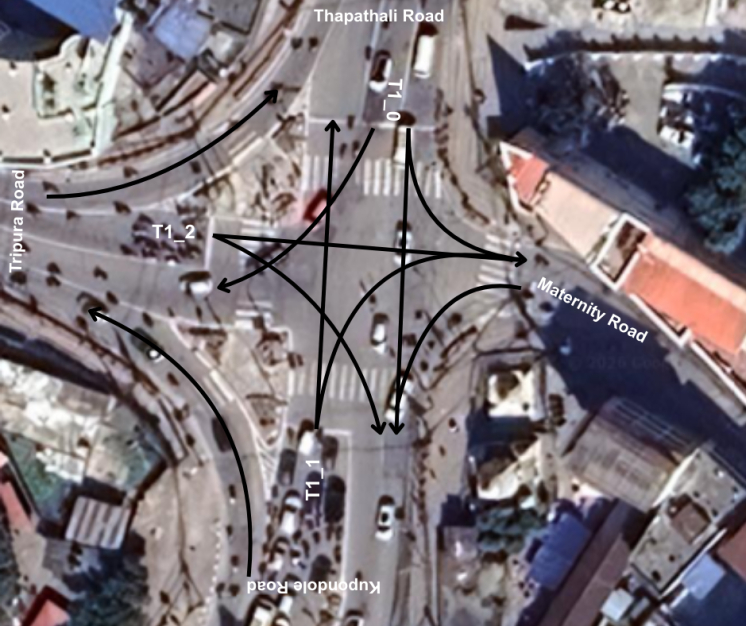
\includegraphics[width=0.8\textwidth]{src/images/figures/traffic_flow_representation.jpeg}
    \caption{Thapathali Road Traffic flow and Traffic light control stage representation}
    \label{fig:traffic_flow_representation}
\end{figure}


    \textbf{Traffic Flow from Tripura Marg} \\
    Vehicles approaching from Tripura Marg have the following movement options:
    \begin{itemize}
        \item Bypass to Thapathali Road (free-flow movement without signal control)
        \item Straight movement to Maternity Road via signal phase T1\_2
        \item Right turn to Kupondole Road via signal phase T1\_2
    \end{itemize}

    \textbf{Traffic Flow from Kupondole Road} \\
    Vehicles entering from Kupondole Road can proceed as follows:
    \begin{itemize}
        \item Bypass to Tripura Marg (uncontrolled/free movement)
        \item Right turn to Maternity Road via signal phase T1\_1
        \item Straight movement (continuation) via signal phase T1\_1
    \end{itemize}

    \textbf{Traffic Flow from Maternity Road} \\
    Vehicles approaching from Maternity Road have:
    \begin{itemize}
        \item Left turn to Kupondole Road
    \end{itemize}

    \textbf{Traffic Flow from Thapathali Road} \\
    Vehicles from Thapathali Road are allowed the following movements:
    \begin{itemize}
        \item Right turn to Tripura Marg via signal phase T1\_0
        \item Left turn to Maternity Road via signal phase T1\_0
        \item Straight movement to Kupondole Road via signal phase T1\_0
    \end{itemize}

\textbf{Signal Phase Representation}
\label{sec:signal-phase-representation}

The signal phase identifiers T1\_0, T1\_1, and T1\_2 represent distinct traffic light control stages within the intersection. Each phase governs a specific set of movements from a particular approach, ensuring orderly and conflict-free traffic flow. These phase labels are commonly used in traffic simulation environments such as \gls{sumo} to define internal connection paths and coordinate signal timing with vehicle movements.

\subsection{Signal Phase Design at Thapathali Intersection}

The traffic signal system at the Thapathali Intersection is organized into three primary movement groups: T1\_0, T1\_1, and T1\_2. These represent distinct sets of directional flows (left, through, right) that are activated in different signal phases. The system operates under three main phase configurations: P0, P1, and P2, where each phase determines which movements are allowed (green) and which are restricted (red).

\begin{figure}[H]
    \centering
    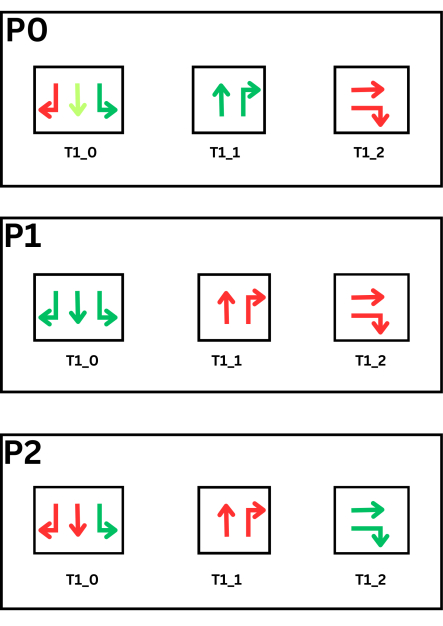
\includegraphics[width=0.8\textwidth]{src/images/figures/implemented_signal_phases.jpeg}
    \caption{Implemented Traffic Signal Phases for fixed-timer and DQN-based Agent}
    \label{fig:implemented_signal_phases}
\end{figure}

\textbf{Traffic Signal Phases}

   \textbf{Phase P0} \\
    In Phase P0, traffic flow is primarily allowed from T1\_1, while movements from T1\_2 are fully restricted and T1\_0 is partially permitted.
    \begin{itemize}
        \item \textbf{T1\_1 (Active -- Green):} Vehicles are allowed to move straight to Thapathali Road and turn right to Maternity Road.
        \item \textbf{T1\_0 (Partially Active):} Only selected straight movements are allowed to Kupondole Road and left movements to Maternity Road. The light green indicates it must wait for vehicle flow to Maternity Road if present, while right-turning movement is restricted to avoid crossing conflicts with T1\_1 flows.
        \item \textbf{T1\_2 (Inactive -- Red):} All movements are stopped via signal phase T1\_2.
    \end{itemize}

   \textbf{Phase P1} \\
    Phase P1 provides \textbf{full priority to T1\_0}, allowing all directional movements, while completely restricting T1\_1 and T1\_2.
    \begin{itemize}
        \item \textbf{T1\_0 (Fully Active -- Green):} Vehicles can perform through movements and right turns freely to Maternity Road and Kupondole Road, respectively. This enables traffic from Thapathali Road to distribute in all directions, including toward Tripura Marg, Maternity Road, and Kupondole Road.
        \item \textbf{T1\_1 (Inactive -- Red):} All movements are stopped via Signal Phase T1\_1.
        \item \textbf{T1\_2 (Inactive -- Red):} All movements are stopped via Signal Phase T1\_2.
    \end{itemize}
\textbf{Phase P2} \\
    Phase P2 shifts priority to \textbf{T1\_2}, allowing its movements while restricting others.
    \begin{itemize}
        \item \textbf{T1\_2 (Active -- Green):} Vehicles are allowed to move straight to Maternity Road and turn right to Kupondole Road.
        \item \textbf{T1\_0 (Partially Active):} Some right turn movements to Maternity Road are permitted depending on conflict-free conditions, while others are restricted.
        \item \textbf{T1\_1 (Inactive -- Red):} All movements are stopped via Signal phase T1\_1.
    \end{itemize}

\textbf{Traffic Signal Control Strategies}

In the fixed-time baseline, the signal follows a 60-second cycle. Phases
P0, P1, and P2 are activated in sequence with predefined allocations.
This is simple to implement and useful as a baseline, but it does not
look at the queue state before deciding whether to hold or change phase.

The DQN controller uses the same phase order but changes how long a phase
is held. Every 15 seconds, it reads the current state and chooses STAY or
NEXT. This keeps the action safe and inspectable while still allowing the
controller to react when demand shifts between approaches.

Downstream backspill was approximated by placing random-timer signals at
the end of outgoing routes. These timers used 30, 45, or 60-second green
durations and included a 3-second yellow transition when movement changed
from green to red. This is not a full downstream network model, but it
prevents outgoing links from behaving as if they had unlimited capacity.
The Maternity road signal was kept fixed at 45 seconds green and 15
seconds red in both controller modes.

% Neural network architecture and learning mechanics of the DQN agent
\section{DQN Agent Implementation}
\label{sec:dqn_agent}

The neural network processed 21-dimensional state inputs through three hidden layers: 128 neurons in the first layer, 64 neurons in the second layer, and 32 neurons in the third layer, all using ReLU activation. The output layer produced 2 Q-values, one for each possible action - STAY and NEXT.

Two networks were maintained. The Q-network selected actions and was
updated during training. The target network provided more stable target
values and copied the Q-network weights every 10 episodes. Experience
replay stored up to 10,000 transitions and sampled mini-batches of 64,
so each update was not based only on the most recent few simulation
steps.

$\epsilon$-greedy exploration began with random actions
($\epsilon = 1.0$). After each episode, $\epsilon$ was multiplied by
0.985 until it reached 0.01 near the end of training. Current Q-values
came from the Q-network, while target values used the Bellman update with
discount factor $\gamma = 0.95$. The difference between the current and
target Q-values was minimised using Adam with a learning rate of 0.001.

% Episode-level training loop, checkpoint saving, and epsilon decay schedule
\section{Training Pipeline Implementation}
\label{sec:training_pipeline}

Training ran for 300 episodes. In each episode, the simulation was reset,
the initial state was read, and the agent selected actions using the
$\epsilon$-greedy policy. When the action changed the phase, a 3-second
yellow interval was applied before the next 15-second green period. The
environment then returned the averaged reward, next state, and episode
metrics. Once the replay buffer contained enough samples, the agent
trained on random mini-batches of 64 transitions.

Between episodes, $\epsilon$ decayed by 0.985. The target network was
updated every 10 episodes, and checkpoints were saved every 5 episodes.
The outputs from training were the saved model, intermediate checkpoints,
and plots for reward, loss, average waiting time, throughput, and epsilon
decay.

% Centralized configuration file managing hyperparameters, file paths, and phase definitions
\section{Configuration Management}
\label{sec:config_management}

The configuration file kept the experiment parameters in one place:
episodes, learning rate, batch size, $\epsilon$ decay, discount factor,
replay buffer size, target-network update frequency, signal identifiers,
lane lists, PCU values, reward weight $\lambda$, SUMO paths, and action
durations. Keeping these values outside the main environment and agent
classes made the training, evaluation, and fixed-baseline scripts use the
same settings.


\section{Metric Calculation}
\label{sec:metric_calculation}

Three primary metrics were tracked throughout training and evaluation to assess intersection performance.

Average Waiting Time was calculated by collecting the waiting time of all vehicles present on the incoming route lanes at regular intervals throughout each episode. At each metric collection step, the mean waiting time across all observed vehicles was accumulated and divided by the total number of collection steps to produce the episode-level average waiting time in seconds.

Average Queue Length was calculated by recording the number of halting vehicles across all incoming route lanes at each metric collection step. A vehicle was considered halting if it was either fully stopped below the SUMO default threshold of 0.1 m/s or slow-crawling below 1.5 m/s. The mean halting count across all monitored lanes was accumulated and divided by the total number of collection steps to produce the episode-level average queue length in vehicles.

Throughput per Wait Second was calculated as a composite efficiency metric by dividing the total episode throughput by the average waiting time, quantifying how many vehicles were processed per second of average delay experienced at the intersection:

$$\text{Throughput per Wait Second} = \frac{\text{Total Throughput (vehicles)}}{\text{Average Waiting Time (seconds)}}$$

A higher value means that more vehicles were cleared for each second of
average delay. This made it useful for comparing the DQN policy with the
fixed-timer baseline under the same demand.
